\documentclass{report}
\usepackage{listings}
\usepackage[margin=1.0in]{geometry}
\usepackage{graphicx}
\usepackage{hyperref}
\hypersetup{colorlinks=true}
\usepackage[document]{}
\title{EECE.5200 - Homework 1}
\author{Travis Kessler}
\date{16 February 2021}
\begin{document}
	\maketitle
	\newpage

	% \lstset{language=shell}
	\lstset{frame=lines}

	\section*{Accessing Source Code}
	
	Source code is available at: \href{https://github.com/tjkessler/eece5200/tree/main/hw1}{https://github.com/tjkessler/eece5200/tree/main/hw1}
	
	\textit{}
	
	\noindent To compile the source code, navigate to the \textit{hw1} directory, and run "make". Each question's executable, "q1a", "q1b", and "q2a", can then be executed from the terminal. "q1a" and "q1b" will produce graphs using gnuplot, and "q2a" will calculate the number of occurrences and proportion of \textit{y} less than \textit{f(x)}.
	
	\section*{Question 1}
	
	\subsection*{a.}
	
	\begin{figure}[!ht]
		\centering
		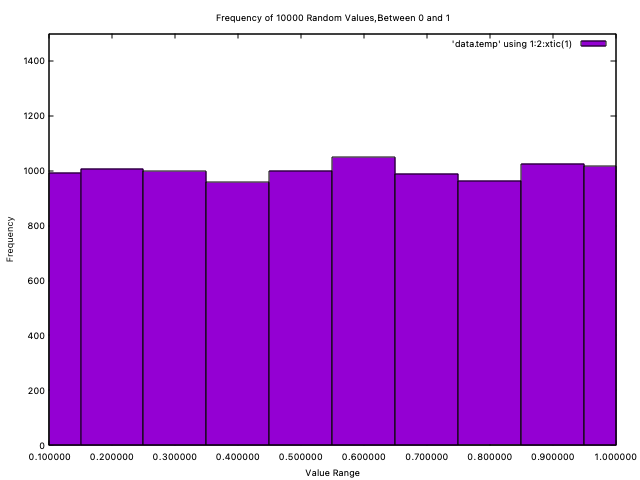
\includegraphics[scale=0.7]{figures/q1a_results.png}
		\caption{Histogram showing uniform distribution of 10,000 RVs generated between 0 and 1}
	\end{figure}

	Figure 1 shows a histogram illustrating the frequency of 10,000 random variables generated between 0 and 1 given 10 histogram bins. It is observed that the histogram is relatively uniform, with each bin containing about 1,000 samples.
	
	\newpage
	
	\subsection*{b.}
	
	\begin{figure}[!ht]
		\centering
		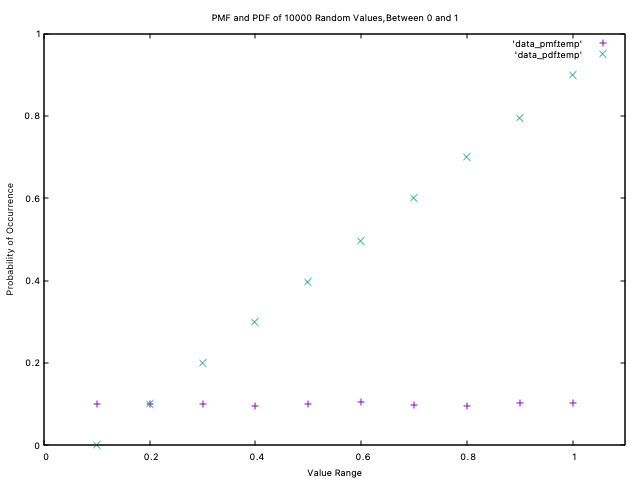
\includegraphics[scale=0.7]{figures/q1b_results.png}
		\caption{PMF and PDF of 10,000 RVs generated between 0 and 1}
	\end{figure}

	Figure 2 shows the probability mass function (purple) and probability density function (teal) of 10,000 random variables generated between 0 and 1 given 10 histogram bins to count frequency. It is observed that each bin of the probability mass function has a probability of ~0.1, and the probability density function increases linearly from 0 to 1.
	
	\newpage
	
	\section*{Question 2}
	
	\subsection*{a.}
	
	Given two uniform random variables \textit{x} and \textit{y}, each with 10,000 samples generated between 0 and 1, and the function \textit{f(x) = x}, it was found that \textbf{5,014} values of \textit{y} are less than \textit{f(x)}.
	
	\subsection*{b.}
	
	Given the linear function \textit{f(x) = x}, it is expected that the integral of \textit{f(x)} from 0 to 1 to be equal to \textbf{0.5} (and subsequently the area equal to 0.5). Based on the number of occurrences of \textit{y} less than \textit{f(x)} found in section a. (5,014) and the total number of samples for the random variable \textit{y} (10,000), the area can be estimated with \textit{5,014 / 10,000}, equaling \textbf{0.5014}.

	\begin{thebibliography}{99\kern\bibindent}
	
	\bibitem{hwref}
	Thompson, C.
	\textit{-1- University of Massachusetts Lowell Department of Electrical and Computer Engineering 16.5200 Computer Aided Engineering Analysis}. Retrieved February 16, 2021, from http://morse.uml.edu/Activities.d/16.520/S2021.d/HW1.pdf
	
	\end{thebibliography}

\end{document}